\documentclass{article}
\usepackage[utf8]{inputenc}
\usepackage{graphicx}

\title{Tittel: Lab 1, Kollisjoner i 2D}
\date{19/09/2024}
\author{Nikolai G. Borbe, Karl-Arne Opkvitne}

\begin{document}

\maketitle

\section*{Hensikt}
\textbf{-> SKRIV INN HER}

\section*{Utstyr}
\begin{itemize}
    \item Kamera: \textit{Panasonic DMC-FZ200}, ID: .
    \item Linse: \textit{DC VARIO-ELMARIT 1:2.8/4.5-108 ASPH.}, ID: .
\end{itemize}

\begin{enumerate}
    \item Setter kamera instillinger til: 100fps HD MP4. Kamera: , Linse: .
    \item Luftbord (Anslått friksjonsfritt)
    \item 2 Pucker
\end{enumerate}

\section*{Beskrivelse}
Vi har 2 pucker med henholdsvis masse $m_1$ og radius $r_1$, og masse $m_2$ og radius $r_2$. Først målte vi de to puckene, for å kunne utføre beregninger ved å ta i bruk de teoretiske formlene.

\begin{figure}[h!]
    \centering
    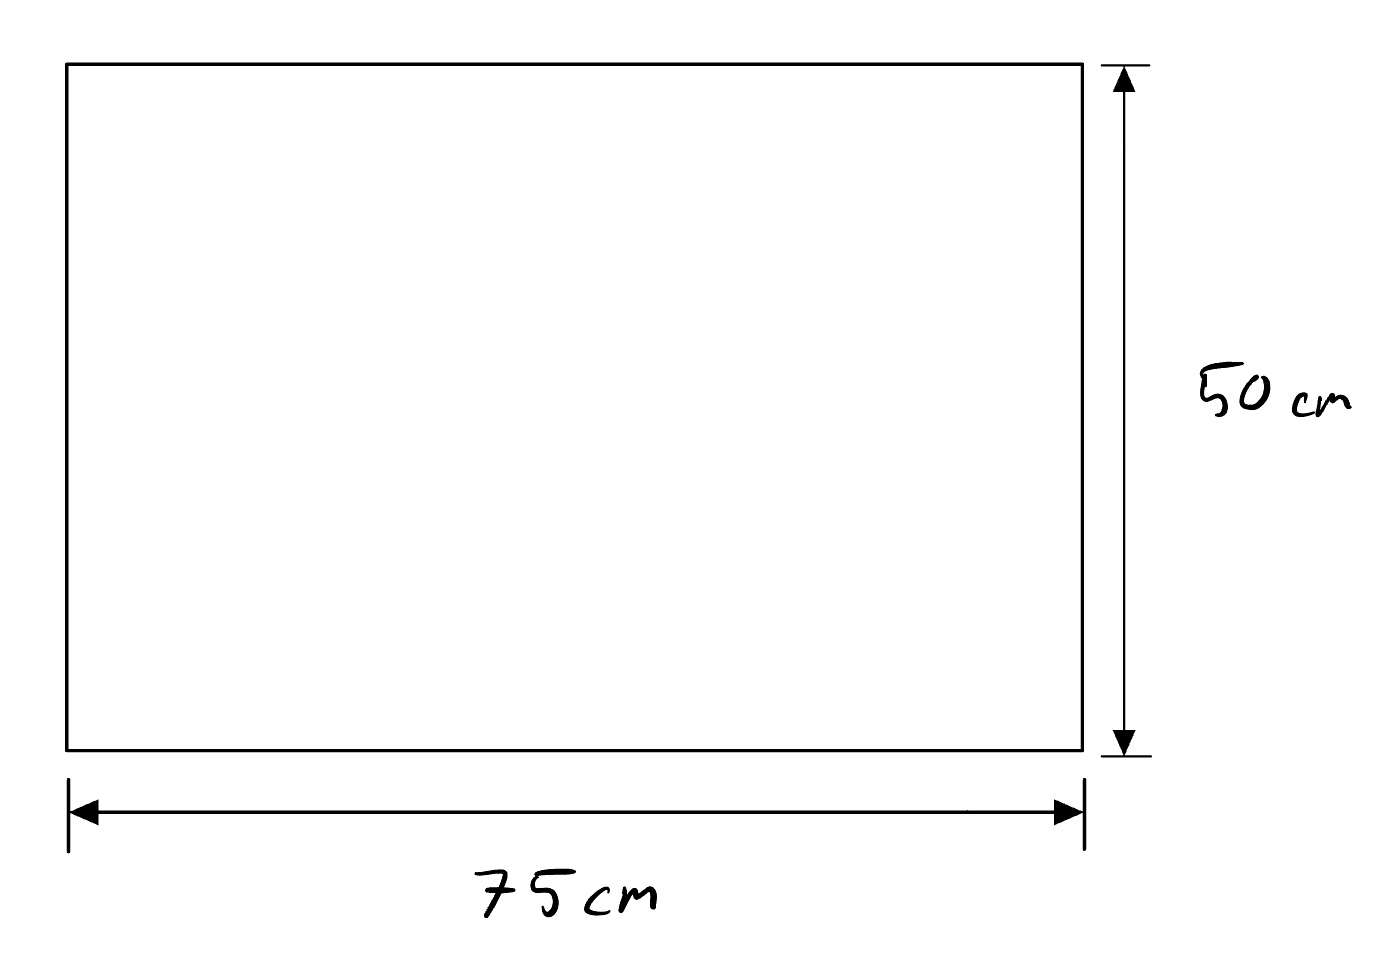
\includegraphics[width=\textwidth]{./images/bord.jpg}
    \caption{Diagram over bord}
\end{figure}

For at friksjonskraften mellom bordet og pucken skulle bli minst mulig hadde vi et "luftbord", altså det ble pumpet luft opp gjennom små hull i bordet slik at kontakten mellom bordet og pucken blir minst mulig.

\begin{figure}[h!]
    \centering
    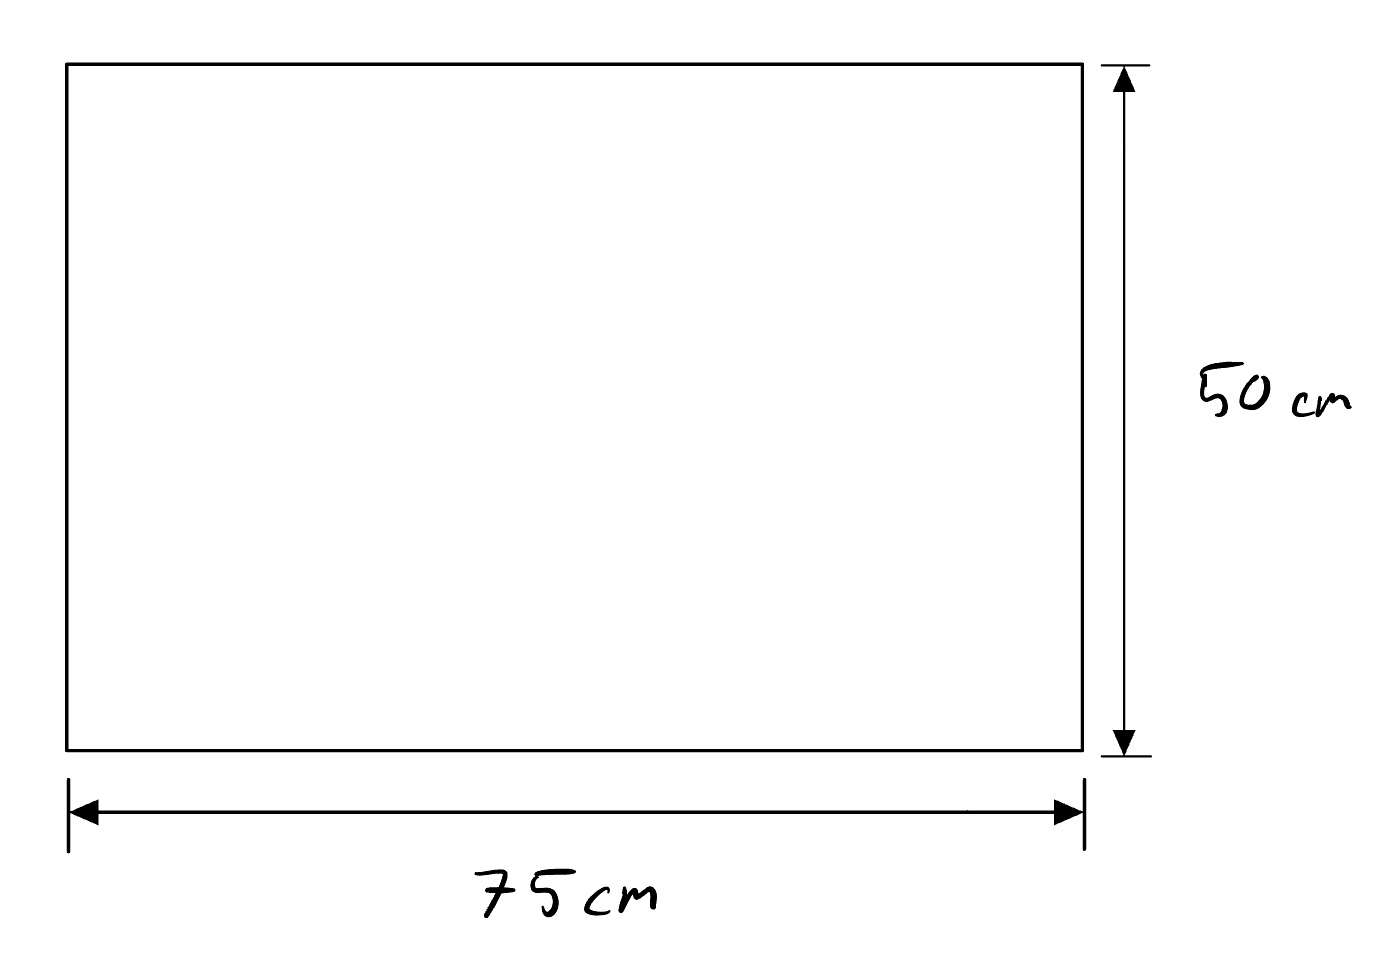
\includegraphics[width=\textwidth]{./images/puck.jpg}
    \caption{Diagram til puck}
\end{figure}

\end{document}
